\documentclass{article}


%\usepackage{PRIMEarxiv}

\usepackage[utf8]{inputenc} % allow utf-8 input
\usepackage[T1]{fontenc}    % use 8-bit T1 fonts
\usepackage{hyperref}       % hyperlinks
\usepackage{url}            % simple URL typesetting
\usepackage{booktabs}       % professional-quality tables
\usepackage{amsfonts}       % blackboard math symbols
\usepackage{nicefrac}       % compact symbols for 1/2, etc.
\usepackage{microtype}      % microtypography
\usepackage{lipsum}
\usepackage{fancyhdr}       % header
\usepackage{graphicx}       % graphics
\graphicspath{{media/}}     % organize your images and other figures under media/ folder
\usepackage{algorithm2e}
\usepackage{subfigure}
%\usepackage{subcaption}
\usepackage{amsmath}
%流程图
\usepackage{tikz}
\usetikzlibrary{arrows, shapes, chains}
\tikzstyle{startstop} = [rectangle,rounded corners, minimum width=3cm,minimum height=1cm,text centered, draw=black,fill=red!30]
\tikzstyle{io} = [trapezium, trapezium left angle = 70,trapezium right angle=110,minimum width=3cm,minimum height=1cm,text centered,draw=black,fill=blue!30]
\tikzstyle{process} = [rectangle,minimum width=3cm,minimum height=1cm,text centered,text width =3cm,draw=black,fill=orange!30]
\tikzstyle{decision} = [diamond,minimum width=3cm,minimum height=1cm,text centered,draw=black,fill=green!30]
\tikzstyle{arrow} = [thick,->,>=stealth]



\newcommand\subtitle[1]{{\small #1}}
\usepackage[colorinlistoftodos]{todonotes}

\hypersetup{
	colorlinks = true, % 使用彩色链接
	linkcolor = blue,  % 链接的颜色
	anchorcolor = blue, % 锚点链接的颜色
	citecolor = blue,   % 引用链接的颜色
	urlcolor = blue,    % URL 链接的颜色
	pdfborder = {0 0 0}, % 取消链接的边框
}

%Header
\pagestyle{fancy}
\thispagestyle{empty}
\rhead{ \textit{ }} 

% Update your Headers here
\fancyhead[LO]{}
% \fancyhead[RE]{Firstauthor and Secondauthor} % Firstauthor et al. if more than 2 - must use \documentclass[twoside]{article}
%opening
\title{Group Project}
\author{}

\begin{document}

\maketitle

\begin{abstract}

\end{abstract}

\section{Introduction}

\section{Related work}

\section{Proposed algorithm: Instance Dependent Cost Online Classification}

In this section, we design heuristics instance-dependent cost in online learning. To simplify cost matrix, we only consider the misclassification cost for each class(degree of freedom: $k^2-k$ down to $k-1$) and the misclassification cost for each instance (degree of freedom: $n\times(k^2-k)$ down to $n\times(k-1)$) , where k is number of classes, n is number of instances. 
\subsection{The original structure of the proposed algorithm}

For each prediction, if our classifier predict correctly, we continue to train the classifier by fitting this instance by the class-dependent cost; Otherwise, i.e. the current classifier can not predict this instance correctly, the instance is difficult to the classifier that it can not handle, our current classifier should pay more attention to this instance. We continue to train the classifier by fitting this instance by the heuristics instance-dependent cost.

Note that in algorithm 1 we take the prediction error into consideration when calculating the heuristics instance-dependent cost. The prediction error term focus more on the instance that p nears to 0.5 but is misclassified as the opposite class. For such instances, our current classifier is almost able to predict correctly, so we give them a higher prediction error cost. However, for the instance that p nears to 0 or 1 but is misclassified as the opposite class, there are two possible reasons: 1) our current classifier is still weak 2) the instance is a noise. For such instance, we give them a lower prediction error cost to prevent overfitting or learning from noise. By receiving the feedback from prediction, the model is trained to strengthen the ability to correctly classify samples that are easy to classify incorrectly, thereby improving the overall performance of the classifier step by step.


\begin{algorithm}
	\caption{Heuristics Instance-dependent Cost Online classification}
	\KwIn{Input data, Input Labels}
	\KwOut{Prediction}
	\While{Have more samples}{
		datum, label <- next sample
		
		prediction label $\hat{y}$  <-  Predict by current classifier
		
		y <- the true label of this sample
		
		current ratio of Class y: $CRC_y$ <- $\frac{\# \ of\ current samples\ with\ label\ y}{\# \ of\ all\ current\ samples}$ 
		
		Class-dependent Cost: $CDC_y$ <- $\frac{1}{CRC_y}$
		
		
		\eIf{Prediction is correct}{
			train the classifier by fitting this instance with the class-dependent cost
		}{
			
			prediction error <- $\alpha e^{\beta (1-y(1-p)-(1-y)p)}$ 
			
			Instance-dependent Cost: $IDC$ <- $CDC_y$ + prediction error 
			
			
			train the classifier by fitting this instance with the heuristics instance-dependent cost
		}
		
		
	}
\end{algorithm}


\subsection{Change the structure of the proposed algorithm}

We have modified the structure of the original algorithm in two aspects, one is the cost of using feedback based on instance prediction results each timestep, and the other one is the modification in the definition of prediction error term.

For the first aspect, we do not distinguish between correctly classified and incorrectly classified instance, using the same definition of instance-dependent cost as the cost for each instance. Since we found that, if the classifier correctly classifies each instance, is will degenerate into class-dependent cost classifier, which shows no obvious difference between class-dependent cost classifier and instance-dependent cost classifier.


For the second aspect, the prediction error is redefined as: 

\begin{equation}
	\text{prediction error} = (1 - p_t)^\alpha,
\end{equation}
 where $p_t$ is the classification probability as the true label, defined as:
 
 \begin{equation}
 	p_t = 
 	\begin{cases}
 		p, \ \text{if y=1}\\
 		1-p, \ \text{if y=0}\\
 	\end{cases}
 \end{equation}
  In the above y $\in$ $\{ 0, 1\}$ specifies the ground-truth class and p $\in$ [0, 1] is the model's estimated probability for the class with label y = 1.

Then the instance-dependent cost is redefined as 
 \begin{equation}
 	\text{instance-dependent cost}= (1+ \text{prediction error})\times \text{class-dependent cost}
 \end{equation}

\begin{figure}[tbh]
	\centering
	\includegraphics[width=1\linewidth]{"in"}
	\caption{instance-dependent cost with different value of $\alpha$}
	\label{fig:instance-dependent-cost-with-different-value-of-alpha}
\end{figure}

The instance-dependent cost is visualized for several values of $\alpha$ $\in$
[0.25, 4] in Figure 1. We note two properties of the instance-dependent cost.
(1) When an instance is misclassified and $p_t$ is small, the
prediction error term nears to 1, which contributes a large instance-dependent cost. As
$p_t$ nears to 1, the prediction error goes to 0 and the instance-dependent cost for well-classified instance is down-weighted to class-dependent cost. (2) The hypothesis parameter $\alpha$ smoothly adjusts the rate at which hard instances are focused on more.

\begin{figure}[h]
	\begin{center}
	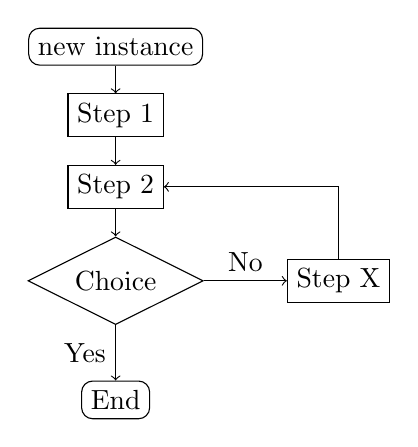
\begin{tikzpicture}[node distance=10pt]
		\node[draw, rounded corners]                        (start)   {new instance
		};
		\node[draw, below=of start]                         (step 1)  {Step 1};
		\node[draw, below=of step 1]                        (step 2)  {Step 2};
		\node[draw, diamond, aspect=2, below=of step 2]     (choice)  {Choice};
		\node[draw, right=30pt of choice]                   (step x)  {Step X};
		\node[draw, rounded corners, below=20pt of choice]  (end)     {End};
		
		\draw[->] (start)  -- (step 1);
		\draw[->] (step 1) -- (step 2);
		\draw[->] (step 2) -- (choice);
		\draw[->] (choice) -- node[left]  {Yes} (end);
		\draw[->] (choice) -- node[above] {No}  (step x);
		\draw[->] (step x) -- (step x|-step 2) -> (step 2);
	\end{tikzpicture}
	\end{center}
	\caption{Flow chart}
\end{figure}


\section{Experiments}

\section{Conclusion}
\end{document}
